\documentclass[11pt, a4paper]{article}

% --- PACKAGES ---
\usepackage[english]{babel}
\usepackage[margin=1in]{geometry}
\usepackage{amsmath, amssymb, amsfonts}
\usepackage{graphicx}
\usepackage{courier} % For typewriter font
\usepackage[colorlinks=true, allcolors=blue]{hyperref}
\usepackage{natbib}
\usepackage{parskip} % Adds space between paragraphs
\usepackage{setspace} % For line spacing
\usepackage{lipsum} % For placeholder text if needed
\usepackage{tikz}
\usetikzlibrary{matrix,positioning,fit,backgrounds}

\linespread{1.1} % Set line spacing

% --- TITLE & AUTHOR ---
\title{Giving Transformers a Blackboard:\\
Can Transformers Learn Algorithms via Spatial reasoning?}
\author{Amir Joudaki \\ \href{mailto:amir.joudaki@inf.ethz.ch}{amir.joudaki@inf.ethz.ch}}
\date{October 7, 2025}

\begin{document}

\maketitle

\section{Introduction}

Modern Large Language Models excel at many tasks, but their reasoning reveals a fundamental weakness: they pattern-match rather than compute. When asked to add two 12-digit numbers, an LLM might guess based on training patterns rather than executing the step-by-step algorithm we learn in elementary school. A calculator that has learned the algorithm can solve exponentially many unseen problems; an LLM often cannot.

\textbf{Can we teach a Transformer to learn an algorithm, not just an empirical distribution?}

You will teach a model to perform multi-digit arithmetic by ``showing its work'' on a 2D ``blackboard.'' This approach builds on Chain-of-Thought (CoT) prompting \citep{wei2022chain}, but extends it to two dimensions: instead of generating a linear trace, our model manipulates symbols on a grid, much like a human would.

While multi-digit addition seems simple, it is a lens for exploring key AI research frontiers: algorithmic reasoning (building models that reliably execute procedures), generalization (training on 5-digit numbers to solve 10-digit problems), interpretability (seeing the algorithm the model has learned), and self-correction (giving the model an ``eraser'' to fix mistakes).

\section{Foundational Concepts and Core Reading}

This project builds on several key areas. You should familiarize yourself with Transformers and the attention mechanism \citep{vaswani2017attention}, which forms the core architecture. The idea of externalizing intermediate reasoning steps through Chain-of-Thought and scratchpads \citep{wei2022chain,nye2021show} is central—our 2D blackboard is a spatially-structured version of this concept.

Understanding how the model perceives symbol locations on a 2D grid is critical for generalization. Review absolute positional encodings in the original Transformer paper \citep{vaswani2017attention}, Rotary Positional Embedding (RoPE) \citep{su2021roformer} for better length extrapolation, and 2D encodings in Vision Transformers \citep{dosovitskiy2020image}. Finally, see how prior work has tested neural networks on algorithmic tasks through benchmarks like those in \citet{saxton2019analysing}.

\section{The Core Task: Building the Blackboard Reasoner}

Your goal is to train a Transformer to solve multi-digit addition by sequentially predicting the next symbol and its location on a 2D grid. The model autoregressively generates the solution one token at a time until completion:

\begin{figure}
\begin{center}
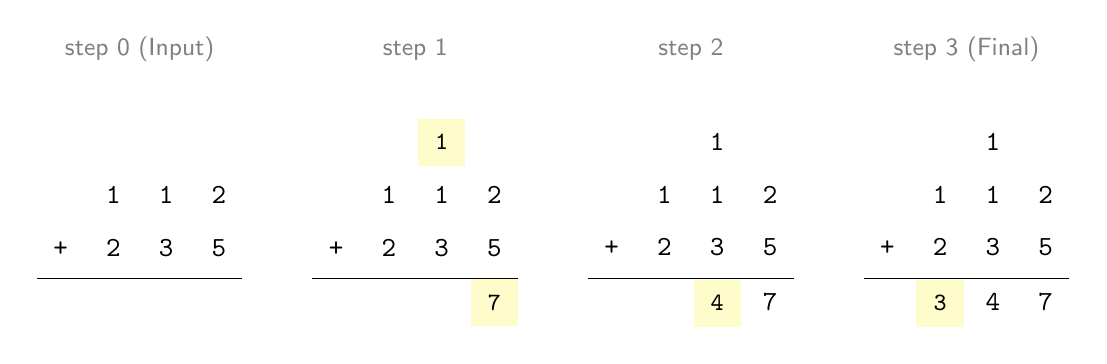
\begin{tikzpicture}[
    cell/.style={minimum width=0.6cm, minimum height=0.6cm, draw=none, font=\ttfamily},
    sstep/.style={font=\small\sffamily, text=gray},
    carry/.style={font=\small\ttfamily, fill=blue!20},
    result/.style={font=\small\ttfamily, fill=yellow!20},
]

% sstep 0
\node[sstep] at (0,2.2) {step 0 (Input)};
\matrix[matrix of nodes, nodes={cell}, column sep=2pt, row sep=2pt] at (0,0) {
&  & & \\
& 1 & 1 & 2 \\
+ & 2 & 3 & 5 \\
\hline
  & & \\
};

% sstep 1
\node[sstep] at (3.5,2.2) {step 1};
\matrix[matrix of nodes, nodes={cell}, column sep=2pt, row sep=2pt] at (3.5,0) {
&  & |[result]| 1 & \\
& 1 & 1 & 2 \\
+ & 2 & 3 & 5 \\
\hline
&  & & |[result]| 7 \\
};

% sstep 2
\node[sstep] at (7,2.2) {step 2};
\matrix[matrix of nodes, nodes={cell}, column sep=2pt, row sep=2pt] at (7,0) {
&  &  1 & \\
& 1 & 1 & 2 \\
+ & 2 & 3 & 5 \\
\hline
 & & |[result]| 4 & 7 \\
};

% sstep 3
\node[sstep] at (10.5,2.2) {step 3 (Final)};
\matrix[matrix of nodes, nodes={cell}, column sep=2pt, row sep=2pt] at (10.5,0) {
 & &  1 & \\
& 1 & 1 & 2 \\
+ & 2 & 3 & 5 \\
\hline
&|[result]| 3 & 4 & 7 \\
};

\end{tikzpicture}
\end{center}
\caption{You can see the transitions from the input to the final stage. At each stage the highlighted cells show where the model made an insertion. }
\end{figure}

\section{Research Directions for Exploration}

After implementing a working baseline, choose one direction to explore in depth.

\paragraph{test/inference time generalization.} How crucial is spatial awareness for learning generalizable algorithms? One key question is positional generalization: does training on 3-digit addition enable solving 5-digit or 10-digit problems (length generalization)? Similarly, does training on top-left problems transfer to bottom-right placement (location generalization)? You should compare different positional encoding schemes—absolute, relative RoPE, and learned 2D encodings—to determine which enables robust generalization. You might also explore whether you can design a positional encoding for unbounded grids, creating a conceptually ``infinite blackboard'' unconstrained by fixed training sizes.

\paragraph{Comparison with CoT.}
A controlled comparison between 1D Chain-of-Thought and your 2D blackboard model will reveal trade-offs in performance, sample efficiency, and generalization.

\paragraph{More complex  operations.}
Can we build a single, general-purpose algorithmic reasoner? Start by training jointly on addition and subtraction to see if the model learns to condition correctly on operators. Compare this multi-task approach to specialized single-task models, and consider extending to multiplication.

Beyond arithmetic, you can explore domain transfer by training on different visual algorithms. Pairwise sequence alignment requires filling dynamic programming tables for edit distance, while Sudoku involves learning constraint satisfaction rules on a grid. For complex tasks, curriculum learning may be essential—starting with simple examples like 2x2 Sudoku before progressing to 4x4. Investigate whether carefully designed curricula enable learning otherwise intractable algorithms.


\paragraph{Giving the model an eraser.} Self-correction is another critical component of robust reasoning. Create a dataset with intentionally corrupted boards (e.g., miscalculated column sums) and train the model to validate state and generate ``eraser'' actions before proceeding. This raises the question: does self-correction improve performance on long reasoning chains where errors compound?


\paragraph{Mechanistic understanding.} Can we have a low level understanding of how the model achieves to implement the algorithm? Mechanistic interpretability offers one approach: analyze attention heads for specialization in sub-tasks. For instance, does one head learn to read column digits while another fetches carry bits? Visualizing attention patterns is a first step toward causal understanding of the learned algorithm.


\section{Practical Notes}

This project is highly feasible. You will train a small Transformer (10M-100M parameters) from scratch on synthetic data—far less resource-intensive than fine-tuning large pre-trained LLMs. You have freedom to choose and justify a suitable architecture: encoder-only, decoder-only, or encoder-decoder configurations each have different strengths for this task.


% --- BIBLIOGRAPHY ---
\bibliographystyle{plainnat}
\bibliography{refs}

\end{document}
